\chapter{Data Model}\label{ch:datamodel}

\figref{fig:datamodel} shows the analysis classes of the data model used by the
application.

\begin{figure}[htb]
	\includegraphics[width=\textwidth]{datamodel}
	\caption{Data model UML diagram (analysis classes).}\label{fig:datamodel}
\end{figure}

\figref{fig:graph} shows a sample snapshot of the database. The following nodes
and relations are defined:
\begin{itemize}
    \item[\textbf{User}] \textit{(node)} Represents a user registered in the
        system. It contains the following properties:
        \begin{itemize}
            \item[\textbf{name}] The name of the user, provided during
                registration;
            \item[\textbf{password}] The hash of the password used by the
                user to log-in;
            \item[\textbf{isOwner}] \textit{(optional)} a boolean value that
                specifies if the user is registered as a restaurant owner or
                as a standard user.
        \end{itemize}
    \item[\textbf{Restaurant}] \textit{(node)} Represents a restaurant. It
        contains the following properties:
        \begin{itemize}
            \item[\textbf{name}] The name of the restaurant;
            \item[\textbf{description}] A textual description of the
                restaurant, provided by the restaurant's owner;
            \item[\textbf{price}] An integer value, which translates to an
                enumerated type, that represents the expensiveness of the
                restaurant.
    \item[\textbf{City}] \textit{(node)} Represents a city. It contains the
        following properties:
        \begin{itemize}
            \item[\textbf{name}] The name of the city;
            \item[\textbf{latitude}] The latitude, used to compute distances;
            \item[\textbf{longitude}] The longitude, used to compute distances.
        \end{itemize}
    \item[\textbf{Cuisine}] \textit{(node)} Represents a cuisine type;
    \item[\textbf{OWN}] \textit{(relation)} Connects a restaurant with his
	    owner;
    \item[\textbf{LOCATED}] \textit{(relation)} Connects a restaurant with the
        city where it is located;
    \item[\textbf{LIVE}] \textit{(relation)} Connects a user with the city where
        he/she lives in;
    \item[\textbf{FOLLOW}] \textit{(relation)} Connects a user with another
	    user.  A user receives recommendations based on the likes of the
	    users he follows;
    \item[\textbf{LIKE}] \textit{(relation)} Connects a user to the
	    restaurants/cuisines that he likes;
    \item[\textbf{SERVE}] \textit{(relation)} Connects a restaurant to all the types
        of cuisine that it serves.
        \end{itemize}
\end{itemize}

\begin{figure}[htb]
    \centering
	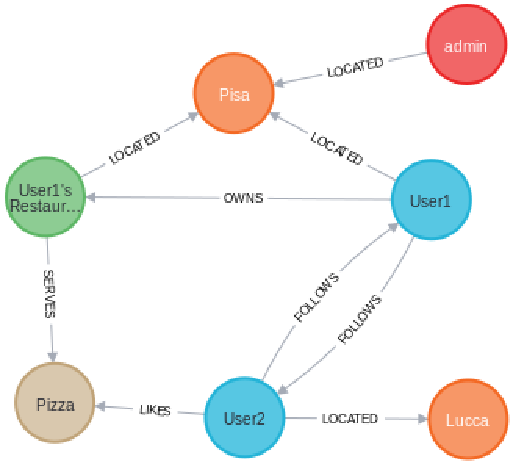
\includegraphics[width=0.8\textwidth]{graph}
	\caption{Graph snapshot.}\label{fig:graph}
\end{figure}

\section{On-Graph Queries}

Four typical ``on-graph'' queries have been defined. The queries allow to
implement the function of restaurant recommendations, user recommendations and
statistics of restaurant of the application on the graph database.

\subsection{Restaurant Recommendations}
\begin{itemize}
    \item [\underline{Domain-Specific Query:}] Find restaurants, which a given
	    user has not liked yet, which are located in a given city, or are
	    located a given number of kilometers from a given city, which make a
	    certain cuisine and which have a certain price. Sort restaurants
	    based on the number of likes of friends, or friends of friends, of
	    the given user.
    \item [\underline{Graph-Centric Query:}] Find the restaurant nodes that have
	    a LOCATED relation with a given city or that have a LOCATED relation
	    with a city whose distance from the given city is under a given
	    number of kilometers, and have a SERVE relation with a given cuisine
	    and with a given value of price attribute. For each resulting
	    restaurant node, count the number of LIKE relation that it has with
	    the user nodes that have a FOLLOW relation to the given user o a
	    FOLLOW relation with user nodes that have a FOLLOW relation with the
	    given user. Sort resulting restaurant nodes for the number of LIKE
	    relation.  
\end{itemize}
    
\subsection{User Recommendations}
\begin{itemize}
    \item [\underline{Domain-Specific Query:}] Find users who are not followed
	    by a given user, who lives in a given city, or lives a certain
	    number of kilometers away from a given city, who likes a certain
	    cuisine.
    \item [\underline{Graph-Centric Query:}] Find the user nodes that have a
	    LIVE relation with a given city or that have a LIVE relation with a
	    city whose distance from the given city is under a given number of
	    kilometers, and have a LIKE relation with a given cuisine and the
	    given user does not have a FOLLOW relation with them.
\end{itemize}
    
\subsection{Ranking Restaurant}
\begin{itemize}
    \item [\underline{Domain-Specific Query:}] Given a restaurant, find its
	    position in the ranking of restaurants, sorted by the number of
	    likes received by users, that are located in the same city, or that
	    make the same cuisine of the given restaurant or both.
    \item [\underline{Graph-Centric Query:}] Find restaurant nodes that have a
	    LOCATED relation with the same city node with which the given
	    restaurant has a LOCATED relation or that have a SERVE relation with
	    the same cuisine node with which the given restaurant has a SERVE
	    relation or both of them. For each resulting restaurant nodes and
	    for given restaurant, count the number of LIKE relation that it has
	    with user nodes. Sort the resulting restaurant nodes for the number
	    of LIKE relation and return the position of the given restaurant.
\end{itemize}
    
\subsection{Likes Restaurant}
\begin{itemize}
    \item [\underline{Domain-Specific Query:}] Find the number of users who have
	    liked a certain restaurant.
    \item [\underline{Graph-Centric Query:}] Count the number of user nodes that
	    have a LIKE relation with the specified restaurant.
\end{itemize}


























